\documentclass[border=10pt]{standalone}

\usepackage{tikz}
\usepackage{tikzsymbols}
\usetikzlibrary{calc,patterns,shapes.geometric}

\def\centerarc[#1](#2)(#3:#4:#5){\draw[#1] ($(#2)+({#5*cos(#3)},{#5*sin(#3)})$) arc (#3:#4:#5);}

\begin{document}
	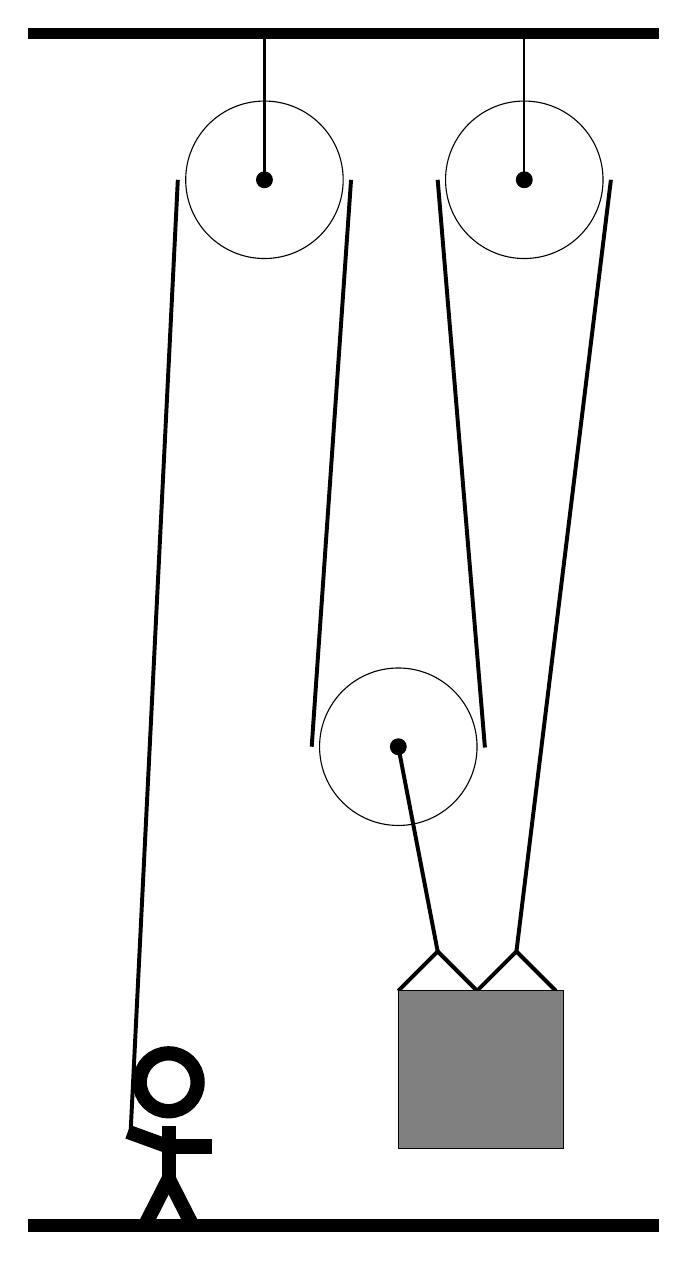
\begin{tikzpicture}
		%%%%% START %%%%%
		\draw[fill=black] (-2, 12) rectangle (6, 12.125);
		
		\draw (1, 10.2) circle (1);
		\draw[fill=black] (1, 10.2) circle (0.1);
		\draw[thick] (1, 10.2) -- (1, 12);
		
		\draw (4.3, 10.2) circle (1);
		\draw[fill=black] (4.3, 10.2) circle (0.1);
		\draw[thick] (4.3, 10.2) -- (4.3, 12);
		
		\draw (2.7, 3.0) circle (1);
		\draw[fill=black] (2.7, 3.0) circle (0.1);
		
		\draw[line width=0.5mm]  (2.7, -0.1) -- (3.2, 0.4) -- (3.7, -0.1) -- (4.2, 0.4) -- (4.7, -0.1);
		\draw[fill=black!50] (2.7, -0.1) rectangle (4.8, -2.1);
		
		\draw[line width=0.5mm](-0.7, -1.9) -- (-0.1, 10.2);
		\centerarc[line width=0.5mm](1, 10.2)(0:180:1.1);
		\draw[line width=0.5mm](2.1, 10.2) -- (1.6, 3.0);
		\centerarc[line width=0.5mm](2.7, 3.0)(180:370:1.1);
		\draw[line width=0.5mm] (3.8, 2.99) -- (3.2, 10.2);
		\centerarc[line width=0.5mm](4.3, 10.2)(0:180:1.1);
		\draw[line width=0.5mm](4.2, 0.4) -- (5.4, 10.2);
		\draw[line width=0.5mm] (3.2, 0.4) -- (2.7, 3.0);
		
		\node at (-0.2, -2) {\Strichmaxerl[10][-20][0]};
		
		\draw[fill=black] (-2, -3) rectangle (6, -3.15);
		%%%%% END %%%%%
	\end{tikzpicture}
\end{document}